\documentclass[a4paper,12pt]{article}
\usepackage[utf8]{inputenc}
\usepackage[spanish]{babel}
\usepackage{color}
\usepackage{parskip}
\usepackage{graphicx}
\usepackage{multirow}
\usepackage{listings}
\usepackage{vmargin}
\graphicspath{ {imagenes/} }
\definecolor{mygreen}{rgb}{0,0.6,0}
\definecolor{lbcolor}{rgb}{0.9,0.9,0.9}
\usepackage{epstopdf}


\setpapersize{A4}
\setmargins{2.5cm}       % margen izquierdo
{1.5cm}                        % margen superior
{16.5cm}                      % anchura del texto
{23.42cm}                    % altura del texto
{10pt}                           % altura de los encabezados
{1cm}                           % espacio entre el texto y los encabezados
{0pt}                             % altura del pie de página
{2cm}     

\lstset{
backgroundcolor=\color{lbcolor},
    tabsize=4,    
%   rulecolor=,
    language=[GNU]C++,
        basicstyle=\tiny,
        aboveskip={1.5\baselineskip},
        columns=fixed,
        showstringspaces=false,
        extendedchars=false,
        breaklines=true,
        prebreak = \raisebox{0ex}[0ex][0ex]{\ensuremath{\hookleftarrow}},
        frame=single,
        showtabs=false,
        showspaces=false,
        showstringspaces=false,
        identifierstyle=\ttfamily,
        keywordstyle=\color[rgb]{0,0,1},
        commentstyle=\color[rgb]{0.026,0.112,0.095},
        stringstyle=\color{red},
        numberstyle=\color[rgb]{0.205, 0.142, 0.73},
%        \lstdefinestyle{C++}{language=C++,style=numbers}’.
}


\begin{document}
\title{Resumen de la CNN}
\author{
Christofer Fabián Chávez Carazas \\
\small{Universidad Nacional de San Agustín} \\
\small{Inteligencia Artificial}
}

\maketitle


\section{Convolutional Neural Networks}

Las redes neuronales covolucionales (CNN) son son una clase mejorada de las redes neuronales convencionales, muy efectivas en la
clasificación y reconocimiento de imágenes. Mientras que a las redes de Kohonen, Hopfield, entre otras, se les pasa como entrada
el vector característica de una imagen; a una CNN se le pasa la imagen entera, tal como está, como entrada. Una CNN reconoce
patrones gracias a las matrices de convolución, y forma vectores característica, que al final son procesados para obtener
un vector de salida con las similitudes con todas las clases, y así poder clasificar la imagen.

\section{Convolución}

Una convolución es un operador matemático que convierte dos funciones en una tercera, siendo esta la representación de la magnitud
cuando las dos funciones se superponen. Matemáticamente, la convolución de $f$ y $g$ se denota $f*g$ y se define con la integral:
$$f*g = \int_{-\infty}^{\infty} f(n)g(t-n)dn$$
En una CNN, al estar operando imágenes, no tiene sentido utilizar esta definición. En cambio se utiliza la definición de
convolución discreta:
$$f[m]*g[m] = \sum_{n=-\infty}^{\infty}f[n]g[m-n]$$

\subsection{Convolución en una CNN}

En una CNN existen las llamadas capas de convolución, las cuales aplican la convolución a una matriz o a un conjunto de matrices con diferentes
filtros. En esta etapa se extraen las características de una imagen. La entrada de la capa es la imagen original si es que es la
primero, o una matriz o varias matrices si es que no lo es. Cada capa tiene varios filtros representados por una matriz de convolución, que si
comparamos con las redes neuronales tradiciones, estas matrices vendrían a ser los pesos de la neuronas.
La idea principal es hacer un barrido con la matriz de convolución por toda la matriz de entrada. Si tenemos una matriz 
de entrada $I$ de tamaño $(I_{n},I_{m})$ y nuestra matriz de convolución $K$ de tamaño
$(K_{n},K_{m})$ entonces tendremos una matriz de salida $IK$ de tamaño $(I_{n} - K_{n} + 1,I_{m} - K_{m} + 1)$. Cada
valor $(i,j)$ de la matriz $IK$ se halla con la siguiente fórmula:
\begin{equation}\label{eq:conv}
IK_{(i,j)}=\sum_{a=0}^{K_{n}-1}\sum_{b=0}^{K_{m}-1}K_{(a,b)} * I_{(i+a,j+b)} 
\end{equation}
Estas operaciones se hacen con cada filtro que tenga la capa. En la ecuación \ref{eq:conv} la matriz de entrada $I$ se mantiene
igual, el $K$ se cambia por cada matriz de convolución. La salida son $q$ matrices, siendo $q$ el número de matrices de 
convolución. Cuando la imagen de entrada es en blanco y negro, no hay mucho problema en aplicar la ecuación \ref{eq:conv}, 
pero si la imagen es a colores, entonces tendremos tres matrices de entrada; una para cada canal de la imagen: R, G y B.
Para este caso la fórmula cambiará \cite{Stutz} de la siguiente forma:
\begin{equation}\label{eq:conv2}
IK_{(i,j)}=\sum_{a=0}^{K_{n}-1}\sum_{b=0}^{K_{m}-1}\sum_{d=0}^{D-1} K_{(a,b,d)} * I_{(i+a,j+b,d)}
\end{equation}
Donde $D$ es el número de dimensiones; en el caso de imágenes a color sería 3. Para que la ecuación \ref{eq:conv2} funcione,
los filtros de la capa deben tener el mismo número de dimensiones que la imagen de entrada. Este caso sólo puede suceder en
la primera capa de convolución, ya que la salida de esta capa van a ser matrices de una sola dimensión, lo cual significa que
las siguientes capas de convolución recibirán como entrada una matriz con una sola dimensión.

\section{Función de Activación}

En redes neuronales, una función de activación determina cuánta energía es disparada por una neurona, o si se dispara o no dicha
energía. En general, la suma de la multiplicación de los pesos con las entradas, o \textit{Neta}, es el valor que se le pasa
a la función. Existen varias funciones de activación: Escalón, Sigmoidea, Gaussiana, Simusoidal, entre otras. Pero la función
adecuada para una CNN es la llamada \textit{rectified linear unit (ReLU)}.

\subsection{ReLU}

Esta función se define de la siguiente manera:
$$f(x) = max(0,x)$$
siendo $x$ la \textit{Neta} de una neurona. La función reemplaza todos los valores negativos por 0, e introduce la no linealidad
a la red neuronal. En una CNN, la función \textit{ReLU} se aplica a cada valor de la matriz de salida, para así obtener una
matriz libre de negativos, la cual es la entrada de la siguiente capa.

\section{Spatial Pooling}

El \textit{Spatial Pooling} reduce la dimensionalidad de una matriz. Una función \textit{pooling} con un tamaño de ventana $kxk$
es aplicada a una matriz $NxN$ de manera distribuida, siendo el resultado una matriz de tamaño $\frac{N}{k} x \frac{N}{k}$. 
En la Figura \ref{fig:pool} se muestra la función \textit{max pooling} con una ventana de $2x2$ aplicada a una función de tamaño $4x4$.
La función divide la matriz en 4 ventanas, de las cuales se saca el número más alto y se forma la matriz resultante.

\begin{figure}
 \centering
 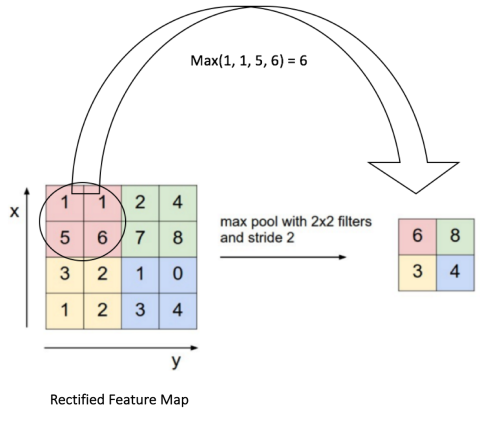
\includegraphics[scale = 0.8]{1.png}
 \caption{Ejemplo de Max Polling \cite{Stan1}}
 \label{fig:pool}
\end{figure}

En una CNN existen las capas de submuestero, que lo único que hacen es aplicar una función \textit{pooling} a la matriz o matrices de entrada. La salida es una matriz ``resumen'' que
representa las características más importantes de la matriz de entrada. Las funciones \textit{pooling} más usadas son: Máximo,
Mínimo, Promedio y Suma. La función Máximo es la recomendada a usar en una CNN.

\section{Fully Connected}

La última capa de una CNN es una tradicional red neuronal multicapa totalmente conectada. La finalidad de esta capa es clasificar
las entradas que le llegan, generando valores de similitud para cada clase de la red. Si la CNN tiene $n$ clases entonces la salida
de la \textit{Fully Conected} tiene $n$ valores. Hay una forma simple de ver esta capa matemáticamente \cite{Stutz}. Tenemos las entradas $I$
con tamaño $(I_{d},I_{n},I_{m})$ siendo $I_{d}$ el número de matrices de entrada, los pesos $W$, y las salidas $z$. Cada valor $i$
de $z$  se calcula con la siguiente ecuación:
\begin{equation}
 z_{i} = \sum_{j=0}^{I_{d}-1}\sum_{r=0}^{I_{n}-1}\sum_{s=1}^{I_{m}}w_{(i,j,r,s)}*I_{(j,r,s)}
\end{equation}
Luego cada valor $z_{i}$ se pasa por una función de activación para que los valores de salida estén entre cero y uno, para luego
poder ver las cercanías con cada clase.

\section{Arquitectura}

Una CNN puede contener varias capas de las ya mencionadas anteriormente. El orden de las capas debe seguir las
siguientes reglas:
\begin{itemize}
 \item Una CNN siempre debe comenzar con una capa convolucional.
 \item Una CNN siempre debe terminar con una capa \textit{Fully Connected} y sólo debe haber una.
 \item Siempre después de una capa convolucional debe ir una de \textit{ReLu}.
 \item Las capas de \textit{pooling} siempre deben ir después de las capas de \textit{ReLu}, pero se pueden omitir.
\end{itemize}

En la Figura \ref{fig:arq} se muestra la arquitectura de una CNN.

\begin{figure}
 \centering
 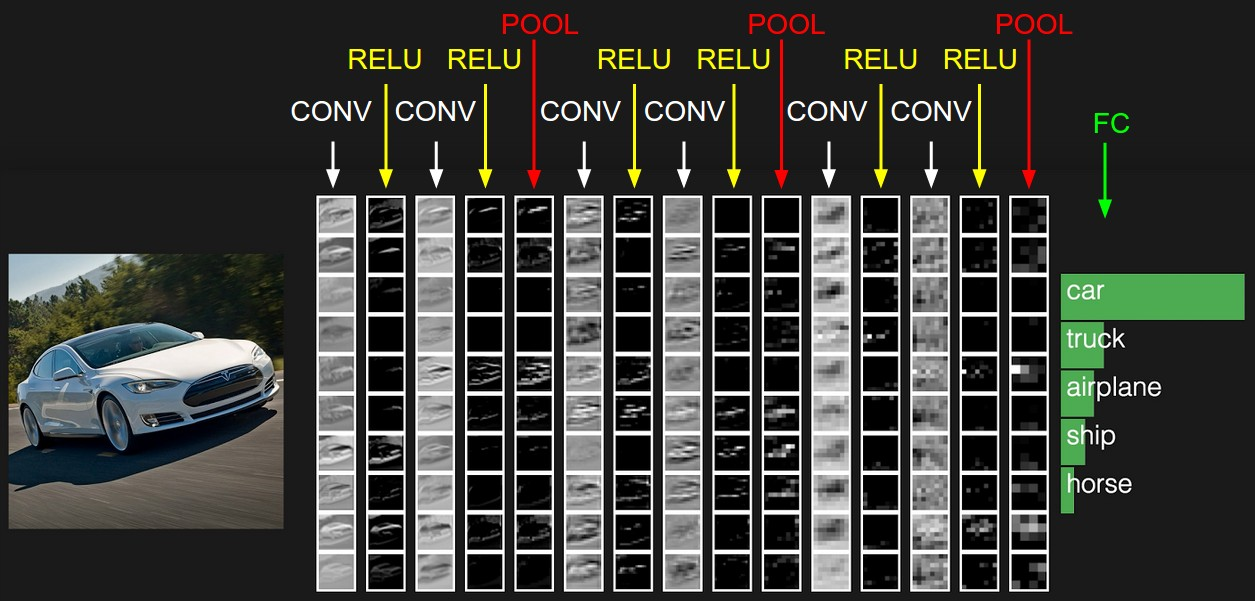
\includegraphics[scale = 0.3]{2.jpeg} 
 \caption{Ejemplo de la arquitectura de una CNN \cite{Stan1}}
 \label{fig:arq}
\end{figure}

\section{Backpropagation}
Para calcular el error de toda la red utilizamos el error cuadrático:
\begin{equation}\label{eq:err}
E = \sum_{p=1}^{P}(\frac{1}{2}(ṭ_{p} - a_{p})^{2})
\end{equation}
donde $P$ es en número de valores de la salida, $t$ es la salida obtenida y $a$ es la salida deseada.
Nosotros queremos minimizar el error de toda la red. Para conseguir esto utilizamos la derivada del error respecto a los
pesos. Para hallar esta derivada tenemos que desmenuzar las derivadas. Tenemos que hallar cómo cambia el error respecto
a la operación de convolución y cómo cambia la operación de convolución respecto a los pesos:
\begin{equation}
\frac{\partial E}{\partial w_{x,y}} = \sum_{x^{'}}\sum_{y^{'}} \frac{\partial E}{\partial o_{x^{'},y^{'}}} \frac{\partial o_{x^{'},y^{'}}}{\partial w_{x^{'},y^{'}}}
\end{equation}
Donde $o$ es la operación de convolución.
Primero veremos la derivada de la operación de convolución respecto a los pesos:

\begin{equation}\label{eq:dvoc1}
\frac{\partial o_{x^{'},y^{'}}}{\partial w_{x^{'},y^{'}}} = \frac{\partial}{\partial w_{x^{'},y^{'}}} (\sum_{x^{''}}\sum_{y^{''}} w_{x^{''},y^{''}} * a_{x^{'} + x^{''},y^{'} + y^{''}})
\end{equation}

\begin{equation}\label{eq:dvoc2}
\frac{\partial o_{x^{'},y^{'}}}{\partial w_{x^{'},y^{'}}} = \frac{\partial}{\partial w_{x^{'},y^{'}}} (w_{0,0} * a_{x^{'} - 0,y^{'} - 0} + \cdots + w_{x,y} * a_{x^{'} - x,y^{'} - y})
\end{equation}

\begin{equation}\label{eq:dvoc3}
\frac{\partial o_{x^{'},y^{'}}}{\partial w_{x^{'},y^{'}}} = \frac{\partial}{\partial w_{x^{'},y^{'}}} (w_{x,y} * a_{x^{'} - x,y^{'} - y})
\end{equation}

\begin{equation}\label{eq:dvoc4}
\frac{\partial o_{x^{'},y^{'}}}{\partial w_{x^{'},y^{'}}} = a_{x^{'} - x,y^{'} - y}
\end{equation}

En la ecuación \ref{eq:dvoc1} se muestra la operación de convolución. En la ecuación \ref{eq:dvoc2} se desmenuza las sumatorias.
En la ecuación \ref{eq:dvoc3} se eliminan las constantes. Y en la ecuación \ref{eq:dvoc4} se saca la derivada quedando sólo el valor
de la entrada que multiplica al peso que se le saca la derivada. \par

Ahora hallamos la derivada del error respecto a la convolución. Para lograrlo desmenuzamos la derivada. Tenemos que hallar cómo 
cambia el error respecto a la salida, y cómo cambia la salida respecto a la operación de convolución:

\begin{equation}\label{eq:dvoc5}
\frac{\partial E}{\partial o_{x^{'},y^{'}}} = \frac{\partial E}{\partial a_{x^{'},y^{'}}} \frac{\partial a_{x^{'},y^{'}}}{\partial o_{x^{'},y^{'}}}
\end{equation}

De la ecuación \ref{eq:dvoc5} hallamos la derivada de la salida respecto a la operación de convolución:

\begin{equation}\label{eq:dvoc6}
\frac{\partial a_{x^{'},y^{'}}}{\partial o_{x^{'},y^{'}}} = f^{'}(o_{x^{'},y^{'}})
\end{equation}

El resultado de esta derivada simplemente es la derivada de la función de activación, en nuestro caso sería la derivada
de la función \textit{ReLU}






\begin{thebibliography}{1}
\bibitem{Stan1} CS231n Convolutional Neural Networks for Visual Recognition, Stanford
\bibitem{Stutz} Stutz, David. ``Understanding convolutional neural networks.'' In Seminar Report, Fakultät für Mathematik, Informatik und Naturwissenschaften Lehr-und Forschungsgebiet Informatik VIII Computer Vision. 2014.
\bibitem{Wu}  Jianxin Wu, ``Introduction to Convolutional Neural Networks'', 2017
\bibitem{back} Jefkine, ``Backpropagation In Convolutional Neural Networks'', 2016
\end{thebibliography}


\end{document}
